% ---------------------------------------------------------------
% Generated by FlowTikZ (flowcharts and data charts to LaTeX)
% Every coordinate below is derived from the editor diagram model.
% Safe to edit by hand, but regenerating will overwrite changes.
% ---------------------------------------------------------------

\documentclass[border=8pt]{standalone}
\usepackage[T1]{fontenc}
\usepackage[utf8]{inputenc}
\usepackage{amsmath}
\usepackage{xcolor}
\usepackage{tikz}
\usepackage[american]{circuitikz}

% ---- Colour definitions ----
\definecolor{fc12161C}{HTML}{12161C}
\definecolor{fc1F2933}{HTML}{1F2933}

% ---- Style definitions ----
\tikzset{
  fcnode/.style={
    draw, inner sep=0pt, outer sep=0pt, align=center,
    line join=round, line cap=butt
  },
  fcpath/.style={line join=round, line cap=butt},
  fcedge/.style={line join=round, line cap=butt},
  fclabel/.style={inner sep=1.4pt, outer sep=0pt, align=center},
}
\tikzset{fccircuit/.style={line join=round, line cap=butt,
  /tikz/circuitikz/bipoles/thickness=1, /tikz/circuitikz/tripoles/thickness=1}}

\begin{document}
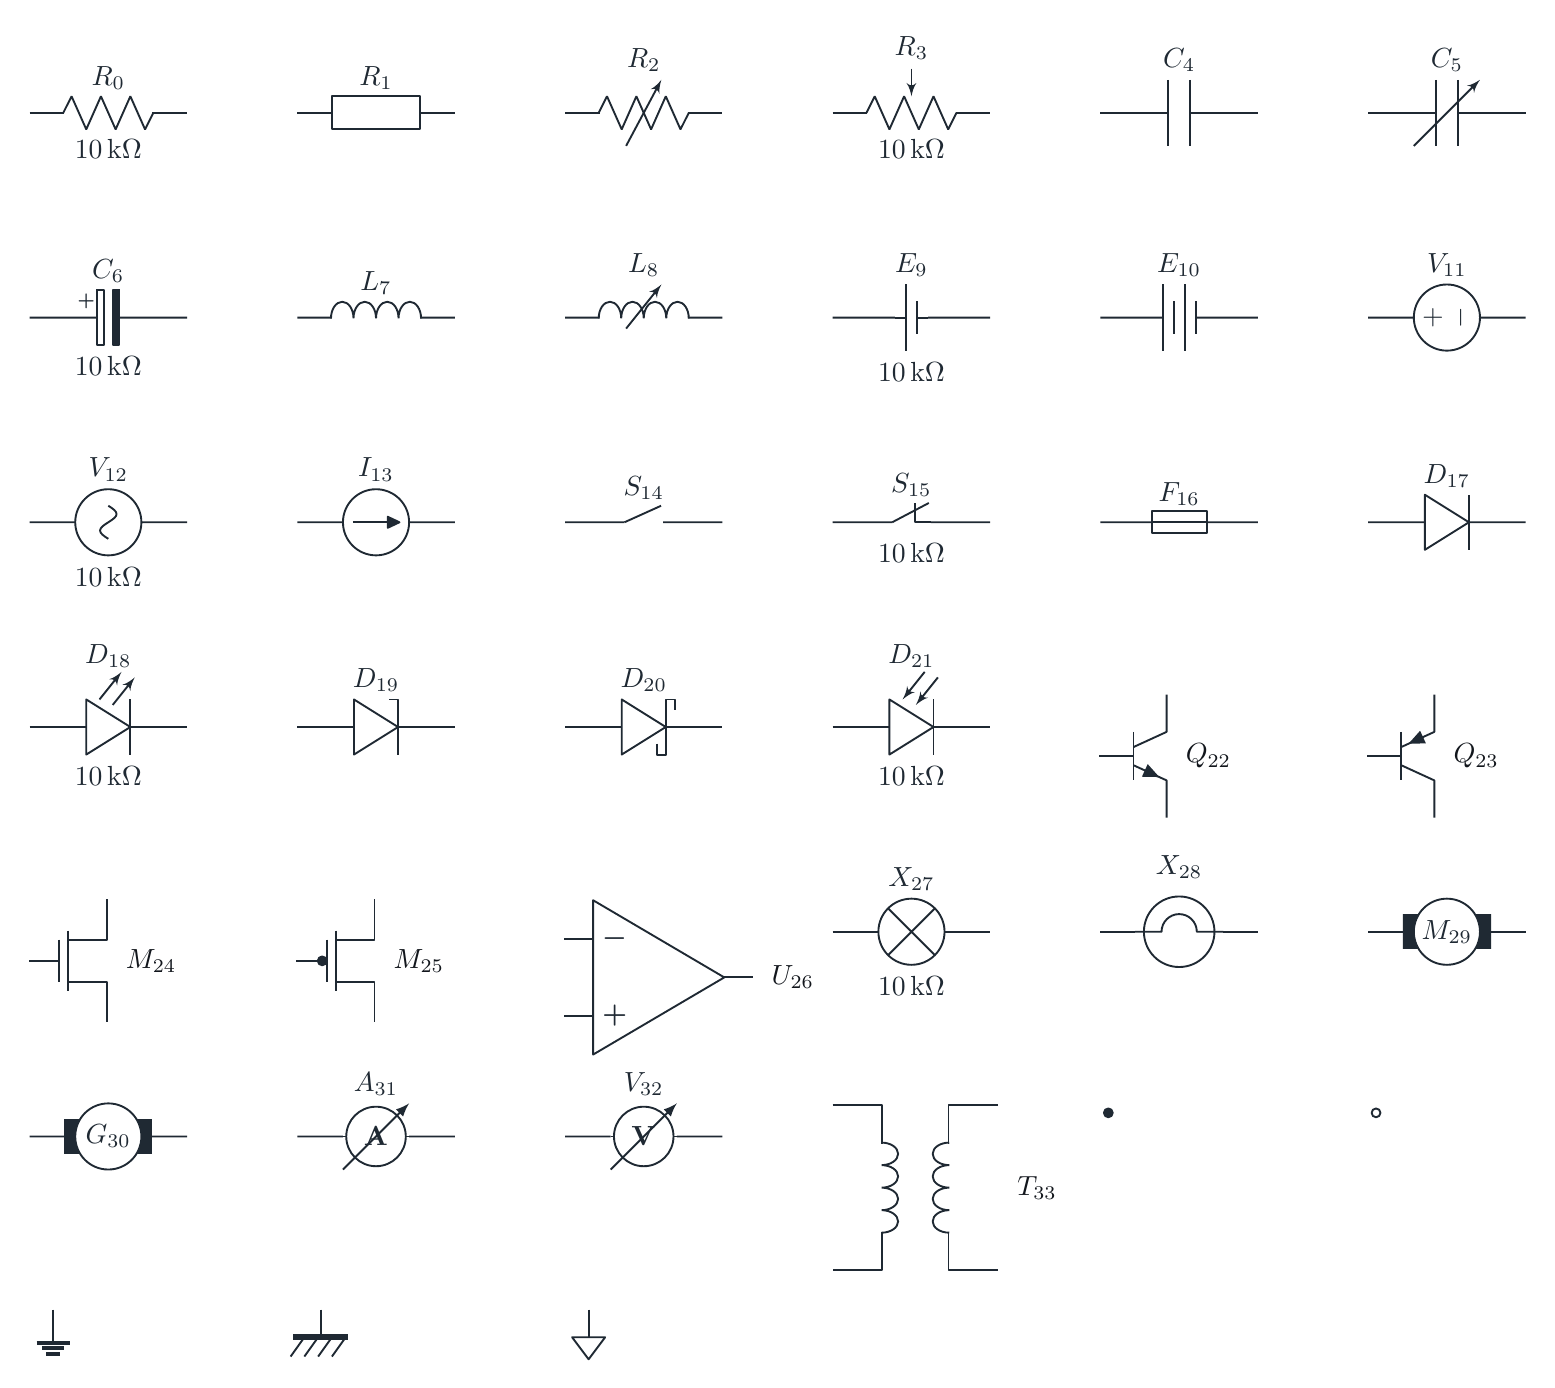
\begin{tikzpicture}[x=1cm, y=1cm]
  % ---- Nodes ----
  % n304 - Resistor "R_{0}"
  \draw[fccircuit, color=fc1F2933, line width=0.683pt, /tikz/circuitikz/bipoles/length=1.4cm]
        (2,-2.4) to[R, l={$R_{0}$}, a={$10\,\mathrm{k\Omega}$}] (4,-2.4);
  % n305 - Resistor (IEC) "R_{1}"
  \draw[fccircuit, color=fc1F2933, line width=0.683pt, /tikz/circuitikz/bipoles/length=1.4cm]
        (5.4,-2.4) to[generic, l={$R_{1}$}] (7.4,-2.4);
  % n306 - Variable resistor "R_{2}"
  \draw[fccircuit, color=fc1F2933, line width=0.683pt, /tikz/circuitikz/bipoles/length=1.4cm]
        (8.8,-2.4) to[vR, l={$R_{2}$}] (10.8,-2.4);
  % n307 - Potentiometer "R_{3}"
  \draw[fccircuit, color=fc1F2933, line width=0.683pt, /tikz/circuitikz/bipoles/length=1.4cm]
        (12.2,-2.4) to[pR, l={$R_{3}$}, a={$10\,\mathrm{k\Omega}$}, name=n307] (14.2,-2.4);
  % n308 - Capacitor "C_{4}"
  \draw[fccircuit, color=fc1F2933, line width=0.683pt, /tikz/circuitikz/bipoles/length=1.4cm]
        (15.6,-2.4) to[C, l={$C_{4}$}] (17.6,-2.4);
  % n309 - Variable capacitor "C_{5}"
  \draw[fccircuit, color=fc1F2933, line width=0.683pt, /tikz/circuitikz/bipoles/length=1.4cm]
        (19,-2.4) to[vC, l={$C_{5}$}] (21,-2.4);
  % n310 - Polarised capacitor "C_{6}"
  \draw[fccircuit, color=fc1F2933, line width=0.683pt, /tikz/circuitikz/bipoles/length=1.4cm]
        (2,-5) to[eC, l={$C_{6}$}, a={$10\,\mathrm{k\Omega}$}] (4,-5);
  % n311 - Inductor / coil "L_{7}"
  \draw[fccircuit, color=fc1F2933, line width=0.683pt, /tikz/circuitikz/bipoles/length=1.4cm]
        (5.4,-5) to[L, l={$L_{7}$}] (7.4,-5);
  % n312 - Variable inductor "L_{8}"
  \draw[fccircuit, color=fc1F2933, line width=0.683pt, /tikz/circuitikz/bipoles/length=1.4cm]
        (8.8,-5) to[vL, l={$L_{8}$}] (10.8,-5);
  % n313 - Cell "E_{9}"
  \draw[fccircuit, color=fc1F2933, line width=0.683pt, /tikz/circuitikz/bipoles/length=1.4cm]
        (12.2,-5) to[battery1, l={$E_{9}$}, a={$10\,\mathrm{k\Omega}$}] (14.2,-5);
  % n314 - Battery "E_{10}"
  \draw[fccircuit, color=fc1F2933, line width=0.683pt, /tikz/circuitikz/bipoles/length=1.4cm]
        (15.6,-5) to[battery, l={$E_{10}$}] (17.6,-5);
  % n315 - DC voltage source "V_{11}"
  \draw[fccircuit, color=fc1F2933, line width=0.683pt, /tikz/circuitikz/bipoles/length=1.4cm]
        (19,-5) to[V, l={$V_{11}$}] (21,-5);
  % n316 - AC voltage source "V_{12}"
  \draw[fccircuit, color=fc1F2933, line width=0.683pt, /tikz/circuitikz/bipoles/length=1.4cm]
        (2,-7.6) to[sV, l={$V_{12}$}, a={$10\,\mathrm{k\Omega}$}] (4,-7.6);
  % n317 - Current source "I_{13}"
  \draw[fccircuit, color=fc1F2933, line width=0.683pt, /tikz/circuitikz/bipoles/length=1.4cm]
        (5.4,-7.6) to[I, l={$I_{13}$}] (7.4,-7.6);
  % n318 - Switch (open) "S_{14}"
  \draw[fccircuit, color=fc1F2933, line width=0.683pt, /tikz/circuitikz/bipoles/length=1.4cm]
        (8.8,-7.6) to[nos, l={$S_{14}$}] (10.8,-7.6);
  % n319 - Switch (closed) "S_{15}"
  \draw[fccircuit, color=fc1F2933, line width=0.683pt, /tikz/circuitikz/bipoles/length=1.4cm]
        (12.2,-7.6) to[ncs, l={$S_{15}$}, a={$10\,\mathrm{k\Omega}$}] (14.2,-7.6);
  % n320 - Fuse "F_{16}"
  \draw[fccircuit, color=fc1F2933, line width=0.683pt, /tikz/circuitikz/bipoles/length=1.4cm]
        (15.6,-7.6) to[fuse, l={$F_{16}$}] (17.6,-7.6);
  % n321 - Diode "D_{17}"
  \draw[fccircuit, color=fc1F2933, line width=0.683pt, /tikz/circuitikz/bipoles/length=1.4cm]
        (19,-7.6) to[D, l={$D_{17}$}] (21,-7.6);
  % n322 - LED "D_{18}"
  \draw[fccircuit, color=fc1F2933, line width=0.683pt, /tikz/circuitikz/bipoles/length=1.4cm]
        (2,-10.2) to[leD, l={$D_{18}$}, a={$10\,\mathrm{k\Omega}$}] (4,-10.2);
  % n323 - Zener diode "D_{19}"
  \draw[fccircuit, color=fc1F2933, line width=0.683pt, /tikz/circuitikz/bipoles/length=1.4cm]
        (5.4,-10.2) to[zD, l={$D_{19}$}] (7.4,-10.2);
  % n324 - Schottky diode "D_{20}"
  \draw[fccircuit, color=fc1F2933, line width=0.683pt, /tikz/circuitikz/bipoles/length=1.4cm]
        (8.8,-10.2) to[sD, l={$D_{20}$}] (10.8,-10.2);
  % n325 - Photodiode "D_{21}"
  \draw[fccircuit, color=fc1F2933, line width=0.683pt, /tikz/circuitikz/bipoles/length=1.4cm]
        (12.2,-10.2) to[pD, l={$D_{21}$}, a={$10\,\mathrm{k\Omega}$}] (14.2,-10.2);
  % n326 - NPN transistor "Q_{22}"
  \node[npn, fccircuit, color=fc1F2933, line width=0.683pt] (n326) at (16.44,-10.57) {};
  \node[anchor=west, text=fc12161C] at (16.56,-10.57) {$Q_{22}$};
  % n327 - PNP transistor "Q_{23}"
  \node[pnp, fccircuit, color=fc1F2933, line width=0.683pt] (n327) at (19.84,-10.57) {};
  \node[anchor=west, text=fc12161C] at (19.96,-10.57) {$Q_{23}$};
  % n328 - N-MOSFET "M_{24}"
  \node[nmos, fccircuit, color=fc1F2933, line width=0.683pt] (n328) at (2.98,-13.17) {};
  \node[anchor=west, text=fc12161C] at (3.1,-13.17) {$M_{24}$};
  % n329 - P-MOSFET "M_{25}"
  \node[pmos, fccircuit, color=fc1F2933, line width=0.683pt] (n329) at (6.38,-13.17) {};
  \node[anchor=west, text=fc12161C] at (6.5,-13.17) {$M_{25}$};
  % n330 - Op-amp "U_{26}"
  \node[op amp, fccircuit, color=fc1F2933, line width=0.683pt] (n330) at (9.99,-13.38) {};
  \node[anchor=west, text=fc12161C] at (11.3,-13.38) {$U_{26}$};
  % n331 - Lamp "X_{27}"
  \draw[fccircuit, color=fc1F2933, line width=0.683pt, /tikz/circuitikz/bipoles/length=1.4cm]
        (12.2,-12.8) to[lamp, l={$X_{27}$}, a={$10\,\mathrm{k\Omega}$}] (14.2,-12.8);
  % n332 - Bulb "X_{28}"
  \draw[fccircuit, color=fc1F2933, line width=0.683pt, /tikz/circuitikz/bipoles/length=1.4cm]
        (15.6,-12.8) to[bulb, l={$X_{28}$}] (17.6,-12.8);
  % n333 - Motor "M_{29}"
  \draw[fccircuit, color=fc1F2933, line width=0.683pt, /tikz/circuitikz/bipoles/length=1.4cm]
        (19,-12.8) to[Telmech=M, l={$M_{29}$}] (21,-12.8);
  % n334 - Generator "G_{30}"
  \draw[fccircuit, color=fc1F2933, line width=0.683pt, /tikz/circuitikz/bipoles/length=1.4cm]
        (2,-15.4) to[Telmech=G, l={$G_{30}$}, a={$10\,\mathrm{k\Omega}$}] (4,-15.4);
  % n335 - Ammeter "A_{31}"
  \draw[fccircuit, color=fc1F2933, line width=0.683pt, /tikz/circuitikz/bipoles/length=1.4cm]
        (5.4,-15.4) to[ammeter, l={$A_{31}$}] (7.4,-15.4);
  % n336 - Voltmeter "V_{32}"
  \draw[fccircuit, color=fc1F2933, line width=0.683pt, /tikz/circuitikz/bipoles/length=1.4cm]
        (8.8,-15.4) to[voltmeter, l={$V_{32}$}] (10.8,-15.4);
  % n337 - Transformer "T_{33}"
  \node[transformer, fccircuit, color=fc1F2933, line width=0.683pt]
        (n337) at (13.25,-16.05) {};
  \node[anchor=west, text=fc12161C] at (14.42,-16.05) {$T_{33}$};
  % n338 - Junction
  \node[circ, fccircuit, color=fc1F2933, line width=0.683pt] (n338) at (15.7,-15.1) {};
  % n339 - Terminal
  \node[ocirc, fccircuit, color=fc1F2933, line width=0.683pt] (n339) at (19.1,-15.1) {};
  % n340 - Ground
  \node[ground, fccircuit, color=fc1F2933, line width=0.683pt] (n340) at (2.3,-17.6) {};
  % n341 - Earth (chassis)
  \node[eground, fccircuit, color=fc1F2933, line width=0.683pt] (n341) at (5.7,-17.6) {};
  % n342 - Signal ground
  \node[sground, fccircuit, color=fc1F2933, line width=0.683pt] (n342) at (9.1,-17.6) {};
\end{tikzpicture}
\end{document}